\section{Hypothesis Testing}
\subsection{Basics}
\textbf{Def 7.1}: A \emph{hypothesis} is a statement about the population distribution.\\
\textbf{Def 7.2}: $H_0$ (null hypothesis) and $H_1$ (alternative hypothesis) are the complementary hypothesis. We write $H_0:\theta\in\Theta_0$ and $H_1:\theta\in\Theta_1$ with $\Theta_k$ mutually exclusive and exhaustive.\\
\emph{Simple} hypothesis: $\Theta_0$ is singleton. \emph{Composite} hypothesis: $\Theta_1$ more than one value.\\
\textbf{Def 7.3}: A \emph{hypothesis test} is a rule when to reject $H_0$ (in favor of $H_1$) given the data. \footnotesize{(\textit{Accepting} $H_0$ is weird, e.g. what about $\theta_0+\epsilon$?.)}\\

\section{Size and Power}
\textbf{T-I error}: Reject $H_0$ although in fact true.\\
\textbf{T-II error}: \emph{Not} reject $H_0$ although in fact false.\\
\textbf{Error rates}: \emph{Probabilities} of making these errors \footnotesize{(errors are random because they depend on the sample)}. Usually \textbf{trade-off} between I and II.\\
% \textbf{I-II-trade-off}: We want to minimize $P_\theta(reject H_0)$ $\forall \theta\in\Theta_0$ and maximize $P_\theta(reject H_0)$ $\forall \theta\in\Theta_1$ \footnotesize{($P_\theta$ denotes probabilities assuming $\theta$ is the true parameter).}\\
\textbf{Def 7.4 (Power function)}: $\beta(\theta) = P_\theta(reject H_0)$.\\
\textbf{T-I error rate}: $\beta(\theta)$ for any $\theta\in\Theta_0$.\\
\textbf{T-II error rate}: $\beta(\theta)$ for any $\theta\in\Theta_1$.\\
\textbf{Def 7.5/7.6}: For $\alpha\in[0,1]$, a test is \emph{level} $\alpha$ if $\sum_{\theta\in\Theta_0}\beta(\theta)\leq\alpha$ (\emph{size}: equality).\\
%\textbf{Test choice}: One approach: fix $\alpha$, take the one with the best power over all $\theta\in\Theta_1$ (might not exist).\\

\subsection{Test statistics and critical values}
\textbf{Goal}: Derive statistic $T$ and reject iff $T>c_\alpha$ controlling $sup_{\theta\in\Theta_0}P_\theta(T>c_\alpha)$ $\Rightarrow$ need $F_T(t)$.\\
\textbf{Ex 7.2 (Two-sided T)}: $X\sim N(\mu, \sigma^2)$ so $\theta = (\mu, \sigma^2)$. Test $H_0:\mu=\mu_0$ against $H_1:\mu\neq\mu_0$ use $T = \frac{\sqrt{n}|\bar{X}_n-\mu_0|}{S_n} ~ |t_{n-1}|$ and reject for $T > c_\alpha = t_{n-1, 1-\alpha/2}$. By construction $sup_{\theta\in\Theta_0}P_\theta(T>c_\alpha)=\alpha$. \footnotesize{Note this holds for all $\sigma^2\in\Gamma$ thus a test of level and size $\alpha$.}\\
\textbf{Ex (One-sided T)}: $T = \frac{\sqrt{n}(\bar{X}_n-\mu_0)}{S_n}$ with $c_\alpha = t_{n-1, 1-\alpha}$ or $Z = -T$ and $c_\alpha$ unchanged (symmetry). Intuition: want to reject for large $\mu > \mu_0$ (right-sided).\\
\textbf{Deriving $\beta(\theta)$}: (1) add and subtract (true) $\mu$, (2) look at behavior as $\mu$ changes. \\
%The one-sided test is also a test for $H_0:\mu\leq\mu_0$ against $H_1:\mu>\mu_0$ with size $\alpha$, because $sup_{\theta\in\Theta_0, \sigma\in\Gamma}\beta^{1sided}(\theta)\leq\alpha$.
% 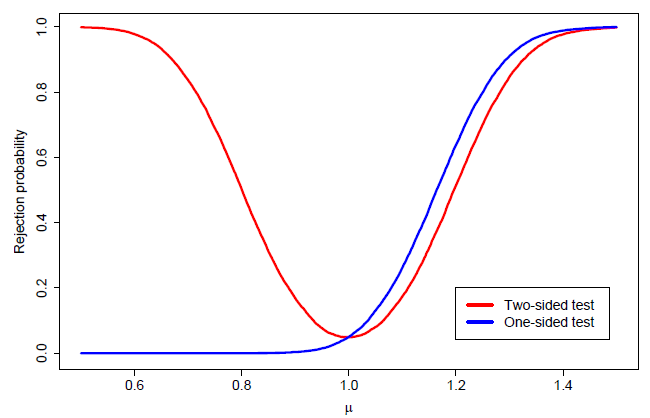
\includegraphics[width = 0.15\textwidth]{content/power_curves.png}\\
\textbf{Def (p-value)}: For any realization $T^*$, $p^* = inf\{p\in[0,1]: T^*>c_p\}$. Intuition: smallest $\alpha$ for which we would still reject. \\\footnotesize{Under $H_0$, $p\sim Unif[0,1]$ (require $P(p^*<\alpha)=\alpha$, i.e. want $Pr_\theta(reject H_0) < \alpha$), but holds $\forall\alpha$.}\\
\textbf{p-value with simple $H_0$}: If $F_0$ is strictly increasing, $p* = 1 - F_0(T*)$ (again: $p~_{H_0}Unif[0,1]$).

\footnotesize{With parametric distributions with multiple parameters (e.g. $N(\mu, \sigma^2)$) usually fix one parameter (e.g. $\sigma^2$) resulting in simple test but technically \textit{composite} $H_0$.}

\subsection{Hypothesis Testing and CIs}
\textbf{Test-inversion}: Assume test $H_0: \theta = \theta_0$ (note: this is some $H_0$) and have test s.t. $P_{\theta_0}(reject H_0) = \alpha$ (size $\alpha$). Assume can perform for any $\theta_0 \in \Theta$. Then we have $CS = \{\theta_0\in\Theta: not reject H_0: \theta=\theta_0\}$ with $P_\theta(\theta\in CS) = 1-\alpha$ (\textit{true} $\theta$).\\
We can also do the reverse: From any CS with coverage rate $1-\alpha$ can construct size $\alpha$ test as $reject\Leftrightarrow \theta_0\notin CS$.\\
\textbf{Ex. one-sided CI}: Testing $H_0: \mu = \mu_0$ against $H_1:\mu>\mu_0$ (or $H_0: \mu \leq \mu_0$) for normal case we have $CS = \{\mu_0 \in [\bar{X}_n - \frac{t_{1-\alpha, n-1}}{\sqrt{n}}S_n, \infty)\}$.

\subsection{Asymptotic Approximations}
\textbf{Asymptotic argument}: No parametric model $f_X(x;\theta)$, but, e.g., moments: $H_0: E(X) = \mu$. $T\xrightarrow{d}|N(0,1)|$ and we can use $\Phi^{-1}(x)$ to control $\alpha$ asymptotically. In particular, $P(T>z_{1-\alpha/2})\rightarrow \alpha$ under $H_0$.\\ 
\textbf{Hypotheses}: Set of distributions $\mathcal{P}$ with $\mathcal{P}_0\subset\mathcal{P}$ set of distributions consistent with $H_0$.\\
\textbf{Def 7.7 (Asymptotic power function)}: $\beta^\alpha(P) = lim_{n\to\infty}\beta_n(P)$.\\
\textbf{Def 7.8/7.9}: test with $\beta^a(P)$ is \emph{asymptotic level} $\alpha$ if $sup_{P\in P_0}\beta^a(P)\leq\alpha$ (\emph{size}: equality).\\
\textbf{Def 7.10}: Test \emph{consistent} against alternative $P\in P_1$ if $\beta^a(P) = 1$.\\
\textbf{Example}: $\mathcal{P} = \{P: E(X), E(X^2) < \infty\}$ and $\mathcal{P}_0 = \{P: E(X) = 1\} \subset \mathcal{P}$ and $\mathcal{P}_1: \{P: E(X) \neq 1\} \subset \mathcal{P}$.\\
\textbf{Problem}: $\beta^a(P)$ might not be informative about finite sample (e.g. $H_0:\mu=\mu_0+\epsilon$). 